\section{Modelo de dominio}


Al modelar el dominio, para afirmaciones como\dots

\begin{itemize}
    \item En la universidad hay alumnos, profesores y PAS
    \item Alumnos y profesores tienen algo que ver
    \item Una asignatura tiene un profesor
    \item Un profesor puede impartir varias asignaturas al mismo alumno
\end{itemize}

\noindent se trata de responder a preguntas del estilo\dots

\begin{itemize}
    \item ¿Qué caracteriza a un profesor?
    \item ¿Qué puede hacer un alumno?
    \item ¿Qué es una asignatura?
    \item ¿Cómo se relacionan los alumnos y los profesores?
\end{itemize}

\vspace*{5mm}

\noindent Siendo formales, se define como Modelo de Dominio al

\begin{enfasis}
    ``Modelo conceptual'' de todos los temas relacionados con un problema específico. En él se describen las distintas entidades,
    sus atributos, papeles y relaciones, además de las restricciones que rigen el dominio del problema.

    \href{https://es.wikipedia.org/wiki/Modelo_de_dominio}{Fuente: Wikipedia}
\end{enfasis}

Habitualmente, se utiliza el \textbf{modelo objeto} para realizar esta descripción, pues permite representar el problema
abstrayendomos de los detalles y tecnología de implementación.

\subsection{Modelo objeto}

Un modelo objeto es un \textit{marco de referencia conceptual} en que se establece un conjunto básico de conceptos, la
terminología asociada y el modelo de computación. Por tanto, este conjunto básico de conceptos deberá considerar el sistema de
información como un conjunto de entidades conceptuales (objetos) que interactuan entre sí. \\
El modelo debe ser facilmente legible y comprensible para los profesionales, aunque no necesariamente comprensible para 
los clientes.

\noindent Elementos fundamentales del modelo objeto:
\begin{itemize}
    \item Abstracción
    \item Encapsulación
    \item Objetos y clases
    \item Mensajes
\end{itemize}

\noindent Elementos secundarios:
\begin{itemize}
    \item Tipos
    \item Persistencia
\end{itemize}

\noindent Elementos avanzados:
\begin{itemize}
    \item Jerarquías de generalización y agregación
    \item Polimorfismo y ligadura dinámica
\end{itemize}

\newpage

\subsubsection{Abstracción}

Seguro que sabes lo que es un gato. Es un animal, un mamífero, un felino, un animal doméstico, un animal de compañía\dots
A partir de ahora te consideraré todo un experto en gatos, sabes tanto sobre ellos, ¿verdad?

\begin{wrapfigure}{r}{7cm}
    \centering
    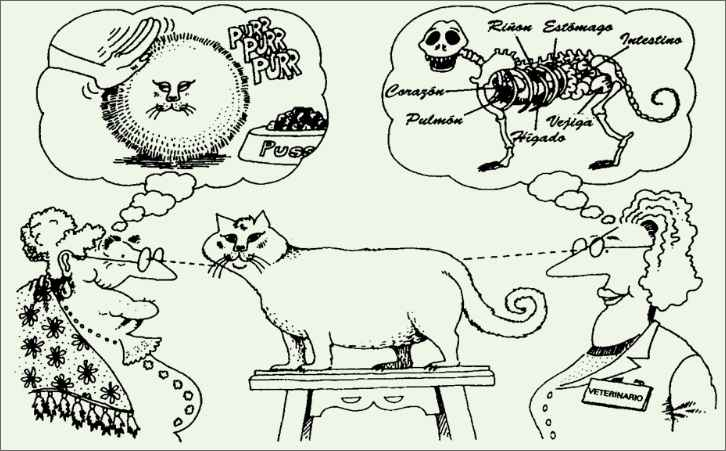
\includegraphics[width=7cm]{assets/Cat1.jpg}
    \caption{¿Qué es un gato?}
    \label{fig:cat1}
\end{wrapfigure}

\vspace*{2.5mm}

\noindent Aunque quizás, quizás no sepas tanto como crees. \textit{¿Qué organos tiene? ¿Cúantos huesos? ¿Cuántos músculos? ¿Estás seguro de que
tiene cualquiera de estas partes?} En esencia, no sabes nada de la implementación de un gato, pero sabes lo que es un gato.
Para la señora de la izquierda, un gato es esa cosa a la que alimentar mucho y acariciar más. Para la de la izquierda, un gato
es un especimen de la familia de los felinos, lleno de complejos y extraños mecanismos biológicos.
Pero, \textbf{ambas dicen saber lo que es un gato}.

\vspace*{2.5mm}

\noindent En el modelo objeto, la \textbf{abstracción} se centra en la visión externa de un objeto, sirviendo para separar su
\textit{comportamiento} de su \textit{implementación}. Esta abstracción es lo que permite centrarnos en las características
esenciales de un objeto, \textbf{en relación al punto de vista de determinado observador}.

Por tanto, no importa saber cuántos músculos tiene un gato, ni cuántos huesos, pues no es relevante a la hora de definir lo que
es. Este es el poder de la abstracción.

\vspace*{2.5mm}

\noindent En definitiva, la \textbf{abstracción} es el elemento básico para combatir la complejidad, y una capacidad indispensable
a la hora de realizar un modelo.

\begin{figure}[h]
    \centering
    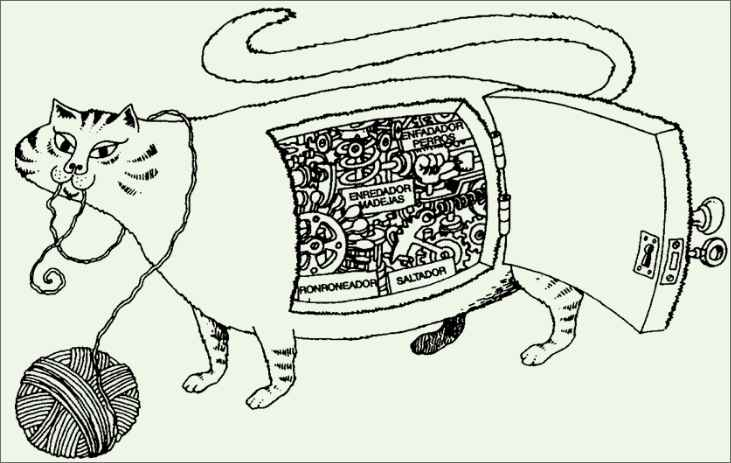
\includegraphics[width=\textwidth]{assets/Cat2.jpg}
    \caption{El verdadero interior de un gato}
    \label{fig:cat2}
\end{figure}

\newpage

Una forma de abstracción es la \textbf{encapsulación}, una técnica de modelado que separa los aspectos externos de un objeto
de los internos (implementación). \textbf{La encapsulación permite ocultar los detalles de implementación de un objeto}. La 
encapsulación crea una barrera \textit{conceptual} que separa la interfaz pública de un objeto de la información y servicios
que contiene.

\subsubsection{Objeto}

\noindent Con el objeto, se modela la permanencia e identidad de conceptos percibidos.
\noindent Se define el objeto como

\begin{enfasis}
    Una entidad definida precisamente con \textbf{identidad}, que encapsula un \textbf{estado} y un \textbf{comportamiento}.
    \begin{itemize}
        \item El \textbf{estado} es representado por sus atributos y relaciones.
        \item El \textbf{comportamiento} es representado por sus métodos y operaciones.
    \end{itemize}
\end{enfasis}

\vspace*{2.5mm}

La identidad es la propiedad que distingue un objeto del resto. No es conveniente que los nombres de los objetos los identifiquen
de forma única:
\begin{itemize}
    \item Un objeto puede no tener un nombre único, y sin embargo ser identificable. Dos gatos pueden tener el mismo nombre,
    pero, \textit{son distintos gatos}.
    \item Un objeto puede tener más de un nombre único. Para la señora de la izquiera, su gato será \textit{Morris}, para mi
    simplemente es \textit{el gato de la señora de la izquierda}, ¡y sigue siendo el mismo gato!.
    \item Un objeto puede cambiar de nombre con el tiempo. La señora de la izquierda adoptó a su gato hace 3 años, era un gato
    callejero, pero en su chapa ponía \textit{Mitens} (maltidos sean sus antiguos dueños), pero a la señora le gustaba mas
    \textit{Morris}, y aún así, de nuevo ¡sigue siendo el mismo gato!
\end{itemize}

\noindent Tampoco los atributos o el comportamiento pueden identificar siempre a un objeto de forma única\dots\space\textit{Morris} tiene un 
hermano gemelo, \textit{Ferris}, luce completamente igual, y además, como se criaron juntos, tienen las mismas costumbres y
comportamiento. Pero estamos fuertemente de acuerdo en que son distintos, ¿no? (ay, ay, ay, que esto se complica\dots).

¿Solución? Es el \textbf{modelo/sistema} quien debe encargarse de la identificación de los objetos.

\vspace*{5mm}

\noindent El \textbf{estado} de un objeto abarca todas las propiedades (estáticas) y sus valores (de caracter dinámico). Además, el estado
incluye las relaciones entre otros objetos. Pero \textbf{OJO}, el \textbf{estado} del objeto no lo identifica, sino su 
\textbf{identidad}.

\vspace*{5mm}

\noindent El \textbf{comportamiento} de un objeto se articula en función de diversos tipos de operaciones:
\begin{enumerate}
    \item Modificador.
    \item Selector.
    \item Iterador.
    \item Constructor.
    \item Destructor.
\end{enumerate}
